%% =====================================================================================
\section{Evaluating the bound}\label{sec:evaluation}
%% =====================================================================================

We now describe how upper bounds $c_p$ for the quantities in \cref{thm:criterion} are computed. There are two
certified computations. The one for \cref{thm:main} ($m=\Mzero$, primes up to $\PmaxMain$) evaluates the comparison
bound exactly, up to truncations whose effect is bounded explicitly (\cref{sec:SBH,sec:tausplit,sec:lost}). The one
for \cref{thm:lean} ($m=\MzeroLean$, primes up to $\Pmax$) uses a cruder evaluation (\cref{sec:AB,sec:theta}), which
was formalized first; the formal proof of \cref{thm:main} evaluates the bounds exactly, for the primes up to $\XFormal$
(\cref{sec:certified-formal}). This section describes the mathematics of the computations; the arithmetic, which
is carried out with directed rounding, is described in \cref{sec:computation} and \cref{app:rounding}.

\subsection{Overview}\label{sec:eval-overview}

For $m=\Mzero$ the checker \code{certificate-14501/src/rigx.c} treats the primes $p\le\PmaxMain$ as follows.
\begin{enumerate}[label=(\alph*)]
\item $p<17$: $\delta_p=0$, and $c_p$ is an upper bound for the first moment $\E[U_p(s)]$ (\cref{sec:eval-M1}).
\item $17\le p<m/2$ ($\nPrimesSBH$ primes, the last one $\lastSBH$): $c_p$ is an upper bound for
  $\E[(U_p(s)-t)^+]/(1-t)$ with $t=\delta_p$, computed from the identity of \cref{lem:SBH}.
\item $m/2<p\le\PmaxMain$: the same quantity, computed from the factorization of \cref{lem:tausplit}.
\end{enumerate}
In (b) and (c) the program also computes the first- and second-moment bounds of \cref{cor:variants}(a),(b) and keeps
the smallest candidate; in the certified run this was the comparison bound at every prime with $\delta_p>0$. The costs
in (b) are then multiplied by $1+2^{-20}$ and those in (c) by $1+2^{-13}$. These deliberate safety margins cost
$4.6\cdot10^{-6}$ in total, and they make the independent checks of \cref{sec:xcheck} strict. The primes $p>\PmaxMain$
are handled by \cref{prop:bbmst61}.

For $m=\MzeroLean$ the checker \code{src/rigcert.c} treats the primes $p\le\Pmax$ as follows.
\begin{enumerate}[label=(\alph*$'$)]
\item $p<31$: $\delta_p=0$ and the first moment.
\item $31\le p\le\PX$: the smallest of upper bounds for $\E[U_p(s)]$, for $\E[U_p(s)^2]/(4d(1-d))$ with
  $d=\min(\delta_p,\frac12)$, and for the comparison bound $\E[(U_p(s)-t)^+]/(1-t)$ for each $t$ in the list
  $\{0.05,0.075,0.1,\dots\}\cap[0,\delta_p)$ together with $t=\delta_p$, evaluated with the decomposition of
  \cref{sec:AB}. In the final run the comparison bound was the smallest at all $\nPrimesCmp$ of these primes, and the
  minimum over $t$ was always attained at $t=\delta_p$.
\item $\PX<p\le\Pmax$: the smallest of the first and second moment bounds and the fractional-moment bounds of
  \cref{cor:variants}(c) for twelve values of $\theta$ (\cref{sec:theta}).
\end{enumerate}
The primes $p>\Pmax$ are handled by the tail estimate of \cref{thm:criterion}.
% CHECK: "the minimum over t was always attained at t = delta_p" is stated in SCRATCH/agents/CONTEXT.md
%        ("verified at all 17,974 primes"); it is not recorded in logs/.  It does not affect the proof.

\subsection{The structure of $U_p$}\label{sec:Ustructure}

Let $N_j=\lceil m/p^j\rceil$ for $j\ge1$. Then $j_0(d)=\min\{j\ge1:d\ge N_j\}$, and $w_p(d)=1/(p-1)$ exactly when
$d\ge N_1$. Writing $c(d)=1-p^{1-j_0(d)}$, which vanishes for $d\ge N_1$, we get
\begin{equation}\label{eq:U-tau}
  (p-1)\,U_p(s)=\tau(s)-\sum_{d\mid s,\ d<N_1}c(d).
\end{equation}
Thus $U_p(s)$ is essentially a divisor count, corrected by the small divisors of $s$. If $p\ge m/2$, then $N_1\le2$,
so $d=1$ is the only divisor that can be below $N_1$: $U_p(s)=\tau(s)/(p-1)$ if $p\ge m$, and
$U_p(s)=(\tau(s)-1+1/p)/(p-1)$ if $m/2\le p<m$, since then $p<m\le p^2$ and $j_0(1)=2$. For small $p$ the correction
in \eqref{eq:U-tau} is substantial, since $N_1$ is large.

\subsection{The first moment}\label{sec:eval-M1}

For the primes with $\delta_p=0$ we use \eqref{eq:EU}: the Euler product $\prod_{q<p}(1+\nu_q/(q-1))$ is rounded up and
the finite sums $\sum_{d<N_j}\nu(d)/d$ are rounded down. The same formula gives the first-moment candidate for larger
$p$. A similar finite formula gives $\E[U_p(s)^2]$ as a $\nu$-weighted sum over pairs of divisors
(\code{src/CERT\_NOTES.md}); it is one of the candidates, but it is never the smallest bound in either certified run.

\subsection{Exact evaluation for $p<m/2$: the S/B/H identity}\label{sec:SBH}

Let $p<m/2$, so that $N_1\ge3$. Choose an integer $y$ with
\begin{equation}\label{eq:ycond}
  y^2\ge N_1,\qquad y\ge N_2,\qquad y\le N_1
\end{equation}
(for instance $y=N_1$; the certified run takes $y=N_1$ if $N_1\le23$, and $y=\max(\lceil\sqrt{N_1}\,\rceil,N_2)$
otherwise). Split the primes $q<p$ into three ranges,
\[
  S=\{q<y\},\qquad B=\{y\le q<\min(N_1,p)\},\qquad H=\{N_1\le q<p\},
\]
write $s=s_Ss_Bs_H$ accordingly, and put
\[
  \tau_S=\tau(s_S),\quad T=\prod_{q\in B\cup H}(v_q+1),\quad F_S=\sum_{d\mid s_S,\ d<N_1}c(d),\quad
  b=\sum_{q\in B,\ v_q\ge1}a_q(s_S),
\]
where $a_q(s_S)=\#\{d\mid s_S:\ dq<N_1\}$.

\begin{lemma}[the S/B/H identity]\label{lem:SBH}
$(p-1)\,U_p(s)=\tau_S\,T-F_S-(1-\frac1p)\,b$.
\end{lemma}

\begin{proof}
Since $\tau(s)=\tau_ST$, by \eqref{eq:U-tau} we must show that $\sum_{d\mid s,\,d<N_1}c(d)=F_S+(1-\frac1p)b$. Let
$d\mid s$ with $d<N_1$, and write $d=d_Sd_Bd_H$ with $d_S\mid s_S$, $d_B\mid s_B$ and $d_H\mid s_H$. Every prime of $H$
is at least $N_1$, so $d_H=1$. Every prime of $B$ is at least $y$, and $y^2\ge N_1$, so $d_B$ has at most one prime
factor counted with multiplicity: $d_B=1$, or $d_B=q$ for a prime $q\in B$ with $v_q\ge1$. The divisors with
$d_B=1$ contribute $F_S$. For a fixed $q\in B$ with $v_q\ge1$, there are exactly $a_q(s_S)$ divisors $d=d_Sq<N_1$
with $d_S\mid s_S$, and each of them satisfies $d\ge q\ge y\ge N_2$, so that $dp^2\ge m$, and $dp<m$, since $d<N_1$.
Hence $j_0(d)=2$ and $c(d)=1-1/p$ for each of them.
\end{proof}

The identity reduces the hinge to three independent pieces: $s_S$, the exponents $(v_q)_{q\in B}$, and $s_H$. The
numbers $a_q(s_S)$ count divisors below $N_1/q\le N_1/y\le y$, so the vector $(a_q(s_S))_{q\in B}$, the
\emph{profile} of $s_S$, depends only on the divisors of $s_S$ below $y$. With $\beta=t(p-1)+F_S+(1-\frac1p)b$,
\[
  \E\bigl[(U_p(s)-t)^+\bigr]=\frac1{p-1}\,\E_{s_S}\Bigl[\tau_S\,\E\bigl[(T-\beta/\tau_S)^+\bigr]\Bigr],
\]
where the inner expectation is over $(v_q)_{q\in B\cup H}$, with $s_S$ fixed. The program evaluates this as follows.
\begin{itemize}
\item It enumerates $s_S$ by a depth-first search over the exponents. A subtree (the exponent of the current prime
  at least $a$, later exponents free) is pruned when the bound
  $\P\cdot\tau\cdot\E[(v+1)\one\{v\ge a\}]\cdot\prod_{\text{later}}\E[v+1]\cdot\E[T]$ for its contribution to
  $\E[\tau_ST]$ is below $10^{-14}\,\E[\tau_S]\E[T]$, and this bound is then added to the result; this is valid
  because $(\tau_ST-\beta)^+\le\tau_ST$.
\item For each profile, it computes the joint law of $(T,b)$ by a dynamic program over the primes of $B$, started
  from the law of $T_H=\prod_{q\in H}(v_q+1)$. The law of $T_H$ is maintained incrementally as $p$ increases; primes
  enter $H$ from both ends, since $N_1$ decreases as $p$ increases.
\item It evaluates each $\E[(T-x)^+;\,b]$ from suffix sums of the law of $T$, by \eqref{eq:suffix} below, with $x$
  rounded down.
\end{itemize}
In the certified run the enumeration visited $143{,}025{,}319$ values of $s_S$ in total; at each level the pruned
part was at most $1.95\cdot10^{-7}$ and the lost mass of \cref{sec:lost} at most $2.19\cdot10^{-6}$ of the level
bound. The identity was first used in the independent recomputation of the certificate for \cref{thm:lean}
(\cref{sec:xcheck}), whose program for these primes makes its own choices of $y$.

\subsection{Exact evaluation for $p>m/2$: the $\tau$-split}\label{sec:tausplit}

Let $p\ge m/2$. By \cref{sec:Ustructure}, $(p-1)U_p(s)=\tau(s)-c_1$ with $c_1=1-1/p$ if $p<m$ and $c_1=0$ if $p\ge m$,
so that $\E[(U_p(s)-t)^+]=\E[(\tau(s)-X)^+]/(p-1)$ with $X=c_1+t(p-1)$. Fix $Y\le p$ (in the certified run
$Y=\firstTau$, the least prime with $N_1\le2$), and write $\tau(s)=\tau_s\tau_l$ with
$\tau_s=\prod_{q<Y}(v_q+1)$ and $\tau_l=\prod_{Y\le q<p}(v_q+1)$, which are independent. For an integer $v\ge0$ let
$f(v)$ be the least integer of the form $2^i3^j$ that is at least $v+1$; thus $f(v)=v+1$ for $v\le3$.

\begin{lemma}[the $\tau$-split]\label{lem:tausplit}
Let $V\ge\tau_l$ be a random variable that depends only on the exponents $v_q$, $Y\le q<p$; for example
$V=\prod_{Y\le q<p}f(v_q)$. Then
\[
  \E\bigl[(\tau(s)-X)^+\bigr]\le\sum_{x}\P(V=x)\,x\,\E\bigl[(\tau_s-X/x)^+\bigr].
\]
\end{lemma}

\begin{proof}
Since $u\mapsto(u-X)^+$ is nondecreasing and $V\ge\tau_l\ge1$, we have
$(\tau_s\tau_l-X)^+\le(\tau_sV-X)^+=V(\tau_s-X/V)^+$. Take expectations, using the independence of $\tau_s$ and $V$.
\end{proof}

The law of $\tau_s$ is computed once, by a dynamic program on $\{1,\dots,2^{22}\}$, together with the suffix sums
that give $\E[(\tau_s-x)^+]$ for every $x$ by \eqref{eq:suffix}. The program takes $V=2^{e_2}3^{e_3}$, obtained from
$\prod_{Y\le q<p}f(v_q)$ by capping $e_3$ at $2$: a factor $3^j$ that would exceed the cap is replaced by
$4^j=2^{2j}$, which is larger. The law of $(e_2,e_3)$ is computed by a dynamic program over the primes in $[Y,p)$,
maintained incrementally in $p$, and states with $e_2>40$ go to the lost mass. Since $\P(v_q\ge4)=\nu_qq^{-4}$ is tiny for $q\ge Y$, the domination $\tau_l\le V$ loses very little. At the
largest primes, however, the threshold $X/V$ can exceed the table of $\tau_s$, and the program then bounds
$\E[(\tau_s-X/V)^+]$ by the lost mass, which is valid but conservative: the referee of \cref{sec:xcheck} found that
this overstates the contribution of the primes above $\PX$ by about $5\cdot10^{-7}$.

\subsection{Truncations and lost mass}\label{sec:lost}

All laws are computed on finite tables with finitely many exponents. Every dynamic program stores upper bounds for the
probabilities of the cells it keeps, and the mass that leaves the tables is not discarded but accounted for as
follows. Let $W$ be the random variable, a product of factors $v_q+1$, whose law is being built, and suppose that a
hinge $\E[(\Lambda W-\beta)^+]$ with $\Lambda,\beta\ge0$ is to be bounded. Split the probability space into the kept
cells and the lost part $L$. On $L$ we use $(\Lambda W-\beta)^+\le\Lambda W$, so that
\[
  \E\bigl[(\Lambda W-\beta)^+\bigr]\le\sum_{\text{kept }w}\P(W=w)\,(\Lambda w-\beta)^++\Lambda\,\E[W;L].
\]
The lost part $E_{\mathrm{lost}}=\E[W;L]$ is accumulated as a sum of nonnegative terms: when a prime $q$ is added,
\begin{equation}\label{eq:lost}
  E_{\mathrm{lost}}\leftarrow E_{\mathrm{lost}}\,\E[v_q+1]+\sum_{w}\P(W=w)\,w\,h(A_w),
\end{equation}
where $h(A)=\E[(v_q+1)\one\{v_q\ge A\}]=\nu_qq^{-A}(A+1+\frac1{q-1})$ and $A_w$ is the least exponent that makes
the cell $w$ leave the table. Cells leave the table when the value
exceeds the table size or the exponent exceeds the cut, and, in the program for \cref{thm:main}, when a cell is
negligible (``dust'', $\P(W=w)\,w<10^{-30}$), in which case its whole contribution $\P(W=w)\,w\,\E[v_q+1]$ is moved to
$E_{\mathrm{lost}}$. The pruned subtrees of \cref{sec:SBH} are treated in the same way. This replaces the formula
$\E[W]-\sum_ww\,\P(W=w)$, which is algebraically identical but suffers from cancellation. Finally, the hinge of a
kept law is evaluated as a sum of nonnegative terms: with the suffix sums $S_0(j)=\sum_{w\ge j}\P(W=w)$ and
$S_1(j)=\sum_{i\ge j}S_0(i)$, and $x'=\lfloor x\rfloor+1$ for $x\ge0$,
\begin{equation}\label{eq:suffix}
  \E\bigl[(W-x)^+\bigr]=\sum_{w\ge x'}(w-x)\,\P(W=w)=S_1(x'+1)+(x'-x)\,S_0(x').
\end{equation}

\subsection{A simpler evaluation for $m=\MzeroLean$}\label{sec:AB}

The certificate for \cref{thm:lean} evaluates the comparison bound for $31\le p\le\PX$ with a decomposition that is
cruder but simpler to formalize. Fix $p$ and $t\in[0,\delta_p]$, let $z=z_p$ be the largest prime $q\le47$ with
$q<\min(p,N_1)$, or $z=1$ if there is none, and split $s=s_As_B$ with $s_A=\prod_{q\le z}q^{v_q}$ and
$s_B=\prod_{z<q<p}q^{v_q}$, which are independent. Let $U_A(s_A)=\sum_{d\mid s_A}w_p(d)$.

\begin{lemma}\label{lem:AB}
$U_p(s)\le U_A(s_A)+(\tau(s_B)-1)\,\tau(s_A)/(p-1)$.
\end{lemma}

\begin{proof}
Every divisor of $s$ is $d_Ad_B$ with $d_A\mid s_A$ and $d_B\mid s_B$. The divisors with $d_B=1$ contribute
$U_A(s_A)$. There are $\tau(s_A)(\tau(s_B)-1)$ others, and each has weight at most $1/(p-1)$.
\end{proof}

The choice of $z$ puts the primes that can divide short divisors into $s_A$; any $z$ gives a valid bound. Let
\[
  G(k,u)=\E_{s_B}\Bigl[\Bigl(u+\frac{(\tau(s_B)-1)k}{p-1}-t\Bigr)^+\Bigr],
\]
which is nondecreasing in $u$ and in $k$. By \cref{lem:AB} and the independence of $s_A$ and $s_B$,
$\E[(U_p(s)-t)^+]\le\E_{s_A}[G(\tau(s_A),U_A(s_A))]$. We split this expectation according to the size of $s_A$:
\begin{multline}\label{eq:AB-bound}
  \E\bigl[(U_p(s)-t)^+\bigr]\le\sum_{s_A\le X_p}\P(s_A)\,G\bigl(\tau(s_A),U_A(s_A)\bigr)\\
  +\sum_{k\le K}R_k\,G\Bigl(k,\frac{k}{p-1}\Bigr)+\frac{\E[\tau(s_A);\tau(s_A)>K]\,\E[\tau(s_B)]}{p-1}.
\end{multline}
Here the first sum runs over all $z$-smooth $s_A\le X_p=\max\bigl(10^4,\,16N_1^{4.5}\bigr)$, which are
enumerated exactly together with $\P(s_A)=\prod_{q\le z}\P(v_q=a_q)$, $\tau(s_A)$ and $U_A(s_A)$; $K=2\cdot10^4$;
and $R_k\ge\P(\tau(s_A)=k,\ s_A>X_p)$. For $s_A>X_p$ we used $U_A(s_A)\le\tau(s_A)/(p-1)$ and the monotonicity of
$G$ in $u$; for $\tau(s_A)=k>K$ we used $G(k,k/(p-1))=\E[(k\tau(s_B)/(p-1)-t)^+]\le k\E[\tau(s_B)]/(p-1)$. (Terms
with $s_A\le X_p$ and $\tau(s_A)>K$ are counted twice, which is harmless.) The numbers $R_k$ are computed as an
upper bound for $\P(\tau(s_A)=k)$, from a dynamic program over the primes $q\le z$, minus a lower bound for the
enumerated mass with $\tau(s_A)=k$. The largest number of enumerated $s_A$ at a single prime was $12{,}114{,}518$.

The function $G$ is evaluated from the law of $\tau(s_B)$. Put $a=k/(p-1)$. If $u\ge t$, then, since $\tau(s_B)\ge1$,
$G(k,u)=u-t+(\E[\tau(s_B)]-1)a$ with $\E[\tau(s_B)]=\prod_{z<q<p}(1+\nu_q/(q-1))$. If $u<t$, then
$G(k,u)=a\,\E[(\tau(s_B)-c)^+]$ with $c=1+(t-u)/a>1$, which is evaluated by \eqref{eq:suffix}. The law of
$\tau(s_B)$ is computed by a dynamic program on $\{1,\dots,10^6\}$, maintained incrementally in $p$: when $p$
increases, the primes in $(z_p,p)$ that are not yet included are added one at a time; since $z_p$ can only decrease
once $p>47$, and $s_B$ is empty for $p\le47$, no prime ever has to be removed. Exponents $a$ with
$\P(v_q=a)<10^{-30}$ or $a>63$ are dropped, and the lost mass is accounted for as in \cref{sec:lost}. The law of
$\tau(s_A)$ and $\E[\tau(s_A);\tau(s_A)>K]$ are computed in the same way, without dropping exponents.

\subsection{Fractional moments for $\PX<p\le\Pmax$ ($m=\MzeroLean$)}\label{sec:theta}

For $p>\PX$ we have $p>m$, so $U_p(s)=\tau(s)/(p-1)$ exactly, and \cref{cor:variants}(c) gives
\[
  c_p=\min_\theta\frac{c_\theta(\delta_p)\,\E[\tau(s)^\theta]}{(p-1)^\theta(1-\delta_p)},\qquad
  \theta\in\{\tfrac32,2,\tfrac52,3,\tfrac72,4,5,6,7,8,10,12\}.
\]
The products $\E[\tau(s)^\theta]=\prod_{q<p}\E[(v_q+1)^\theta]$ are maintained as running products over the primes.
Each factor is computed from \eqref{eq:Etheta}: the series is summed until its terms are negligible, and the
remainder is bounded rigorously, since for $a\ge A+1$ the terms $b_a=q^{-a}(a+1)^\theta$ satisfy
$b_{a+1}/b_a\le r:=((A+3)/(A+2))^\theta/q$, so that $\sum_{a>A}b_a\le b_{A+1}/(1-r)$. Half-integer powers use a
square root rounded in the required direction. At the eleven primes of this range examined in the independent
recomputation, the minimum is attained at $\theta=\frac52$ for $p\le10^7$ and at $\theta=3$ for $p\ge5\cdot10^7$
(\code{tests/xcheck\_final/out/task4\_full.out}). The $\nPrimesC$ primes in this range contribute $\blockC$ in
total, about six times the exact values of their comparison bounds (\cref{sec:reach}).

\subsection{The tail}\label{sec:tail}

\Cref{thm:criterion} with $X\ge2^{27}$ requires an upper bound for
$T_X=\prod_{q\le X}(1+\nu_q(3q-1)/(q-1)^2)$, which the programs compute as a running product, rounded up. Note that
$T_X=\E[\tau(s)^2]$ for the random number $s$ built from all primes $q\le X$. For $m=\MzeroLean$ and $X=\Pmax$ the
tail term in \eqref{eq:criterion} is $\frac{100}{189}T_X/X\le\tailElem$. For $m=\Mzero$ and $X=\PmaxMain$ it would be
about $3.7\cdot10^{-4}$, which exceeds the margin $1-\eta\approx7.3\cdot10^{-5}$; there we use the criterion of BBMST,
which the programs check as well. The formal proof of \cref{thm:main} instead takes $X=\XFormal$ and the constant of
\cref{prop:tailtwo}, which make the tail term $\tailFormal$ (\cref{sec:certified-formal}).

\begin{proposition}[{via \cite[Theorem~6.1]{BBMST}}]\label{prop:bbmst61}
In the setting of \cref{thm:criterion}, suppose instead of \eqref{eq:criterion} that $\eta:=\sum_{p\le X}c_p<1$,
that $k:=\pi(X)\ge10$, and that
\[
  \frac{T_X}{1-\eta}\le(\log k+\log\log k-3)^2\,k .
\]
Then no family of congruences with distinct moduli, all at least $m$, covers $\Z$.
\end{proposition}

\begin{proof}
Following \cite[Section~6]{BBMST}, perform a sieve step at every prime, with the trivial step ($B_i=\emptyset$,
$P_i=P_{i-1}$) at primes not dividing $Q$, and write $p_i$ for the $i$-th prime. With $i_0=0$ and $\kappa=1$,
\cite[(19)]{BBMST} defines $f_k=\mu_k^{-1}\prod_{i\le k}\bigl(1+\nu_{p_i}(3p_i-1)/(p_i-1)^2\bigr)$, where
$\mu_k=1-\sum_{i\le k}P_i(B_i)$. Their hypothesis \cite[(20)]{BBMST} for these $\kappa$ and $i_0$ is the bound
\eqref{eq:bbmst32} of \cite[Theorem~3.2]{BBMST}, valid since all $\delta_q\le\frac12$ (including factors for primes
that do not divide $Q$ only increases the product). By \cref{thm:perprime} and \cref{cor:variants},
$\mu_k\ge1-\eta>0$, so $f_k\le T_X/(1-\eta)$, and \cite[Theorem~6.1]{BBMST} applies. Its proof sets
$\delta_i=\frac12$ for $i>k$ and uses Dusart's bound $p_i\ge i(\log i+\log\log i-1)$ \cite{Dusart1999}.
\end{proof}

\subsection{The distortion schedules}\label{sec:schedule}

For $m=\Mzero$ the schedule is $\delta_q=0$ for $q<17$ and, for $q\ge17$, piecewise linear in $\log q$ through the
$\nKnotsMain$ knots listed in \cref{app:schedule}, from $(17,0.00375)$ to $(2\cdot10^5,0.46)$, and constant $0.46$
beyond; $\delta_q=\frac12$ for $q>\PmaxMain$ in the tail argument. For $m=\MzeroLean$ it is
\[
  \delta_q=\begin{cases}0,& q<31,\\ 0.05,& 31\le q<50,\\
  \text{piecewise linear in }\log q\text{ through the knots of \cref{tab:knots}},& 50\le q\le50{,}000,\\
  0.4092,& q>50{,}000,\end{cases}
\]
for $q\le\Pmax$, and $\delta_q=\frac12$ for $q>\Pmax$. Both are shown in \cref{fig:schedule}(a). They were found by
numerical searches with floating-point versions of the evaluators, and as noted in \cref{rem:any-schedule}, the
certificates do not depend on how they were found. The values actually used by the certified programs differ from
these by rounding (\cref{sec:rounding}).

\begin{figure}[ht]
  \centering
  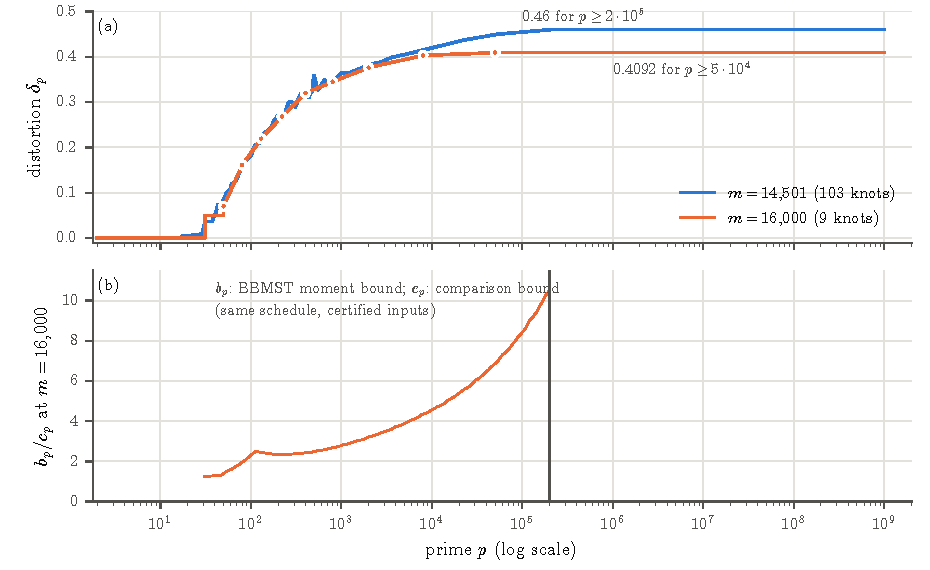
\includegraphics[width=\textwidth]{fig/schedule_gain.pdf}
  \caption{(a) The distortion schedules $\delta_p$ of the two certified runs; the dots are the knots of the schedule
  for $m=\MzeroLean$. (b) The ratio $b_p/c_p$ of the moment bound $b_p=\min\bigl(\E[U_p],\E[U_p^2]/(4\delta_p(1-\delta_p))\bigr)$
  of BBMST to the certified comparison bound $c_p$ at $m=\MzeroLean$, for $31\le p\le\PX$, with the same schedule;
  both are computed from certified quantities.}
  \label{fig:schedule}
\end{figure}

With the same schedule, the comparison bound is smaller than the moment bound of BBMST by a factor between
$\gainAmin$ and $\gainAmax$ for $31\le p<50$, between $\gainBmin$ and $\gainBmax$ for $50\le p<2{,}000$, and between
$\gainCmin$ and $\gainCmax$ for $2{,}000\le p\le\PX$ (\cref{fig:schedule}(b)).
